\documentclass[11pt,a4paper,oneside]{article}
\usepackage[left=2cm,right=2cm,top=2cm,bottom=2cm]{geometry}
\usepackage[document]{ragged2e}
\usepackage[utf8]{inputenc}
\usepackage{amsmath}
\usepackage{amsfonts}
\usepackage{amssymb}
\usepackage{graphicx}
\usepackage{xcolor}
\usepackage{subfig}
\usepackage[output-decimal-marker={.}]{siunitx}
\usepackage{wrapfig}
\usepackage{lipsum}
\usepackage[toc]{appendix}
\usepackage{eso-pic}
\usepackage{hyperref}
\usepackage{siunitx}

\title{%
 \vspace{-2.0cm}
 Exploring Onset Finding Algorithms: A Monte Carlo \\ Simulation For  Hyperfine Splitting Measurement of Anti-Hydrogen
}

\date{\vspace{-5ex}}
\author{Adriano, Simone,Germano }
\begin{document}

\AddToShipoutPicture*
    {\put(520,775){
\includegraphics[width = 0.125\textwidth]{logo/ALPHA_Logo.jpg}}}

\maketitle
\begin{abstract}
\centering
In this report we present a simple Monte Carlo simulation developed within the context of ALPHA-2 Hyperfine Splitting measurement. The objective of this study is to assess the statistical uncertainty and bias of the algorithm utilized in 2017 analysis when applied to the new arrangement of data collected in 2023. In addition to this, different algorithms have been tested, as alternatives of the algorithm used in the previous analysis.
\end{abstract}

\paragraph{Introduction}

The Hyperfine Splitting Measurement consists on the determination of the $\Delta f$ frequency transitions between $c \rightarrow b$ and $ d \rightarrow a$ states of anti-hydrogen. This measure is carried out in ALPHA-2, where the anti-hydrogen is irradiated with the light produced by a laser with variable frequency. Due to the transitions induced by the light, a certain amount of anti-hydrogen is released from the trap and annihilates. The counts of anti-hydrogen annihilation per frequency constitutes the experimental \textit{line-shape}. During the experiment, the \textit{line-shape} of the $c \rightarrow b$ and $ d \rightarrow a$ transitions are measured. The Hyperfine Splitting is determined by the frequency interval between the two \textit{line-shapes}, which is estimated taking the difference of the frequency onset of the two \textit{line-shapes}. This study is done using \textit{ROOT} and \textit{RDataFrame} framework. All the software used for the simulation can be found here: {\color{blue}{\url{https://github.com/Adrianodelvincio/ALPHA.git}}}

\section{High Statistic Line-Shape, Cosmic Background and Annihilation due to Residual Gas}

The simulation developed and discussed in this note has the aim to reproduce the experimental routine to obtained the hyperfine splitting of anti-hydrogen from the series of run collected in 2023 at ALPHA-2 apparatus. It does not account atomic physics and dynamical simulation of trapped anti-hydrogen in order to reproduce the shape of anti-hydrogen transition. Instead, the simulation focuses on the experimental procedure to extract the onsets frequency from the data considering also the most important secondary effects which can influence the measurement.

in this framework, the two transition are $cb$ and $da$ are simulated from model determined to fit the data contained in the high statistic run ... 
We point out that this model is a rough estimation of the true line-shape of the transition. We expect the shape of the transition to be influenced by the power of the microwave laser used to induce it, and the model used to generate the data is only a rough approximation of how the real data look like.

The model used to analyze the high statistic run is a truncated Cruiff function, which is a modified version of a gaussian which accounts for the possibility of having asymmetric tails.

\begin{equation} \label{eq:Cruiff}
mettere \, equazione
\end{equation} 

The parameters of this model are extracted from the fit to the data, and then saved in the configuration file of the simulation. The fit applied is a \textit{Maximum Likelihood fit}, with six free parameters, fixing the value of the $onset$ at $\SI{175}{ \kilo \hertz}$.

\begin{figure}[hbtp]
\centering
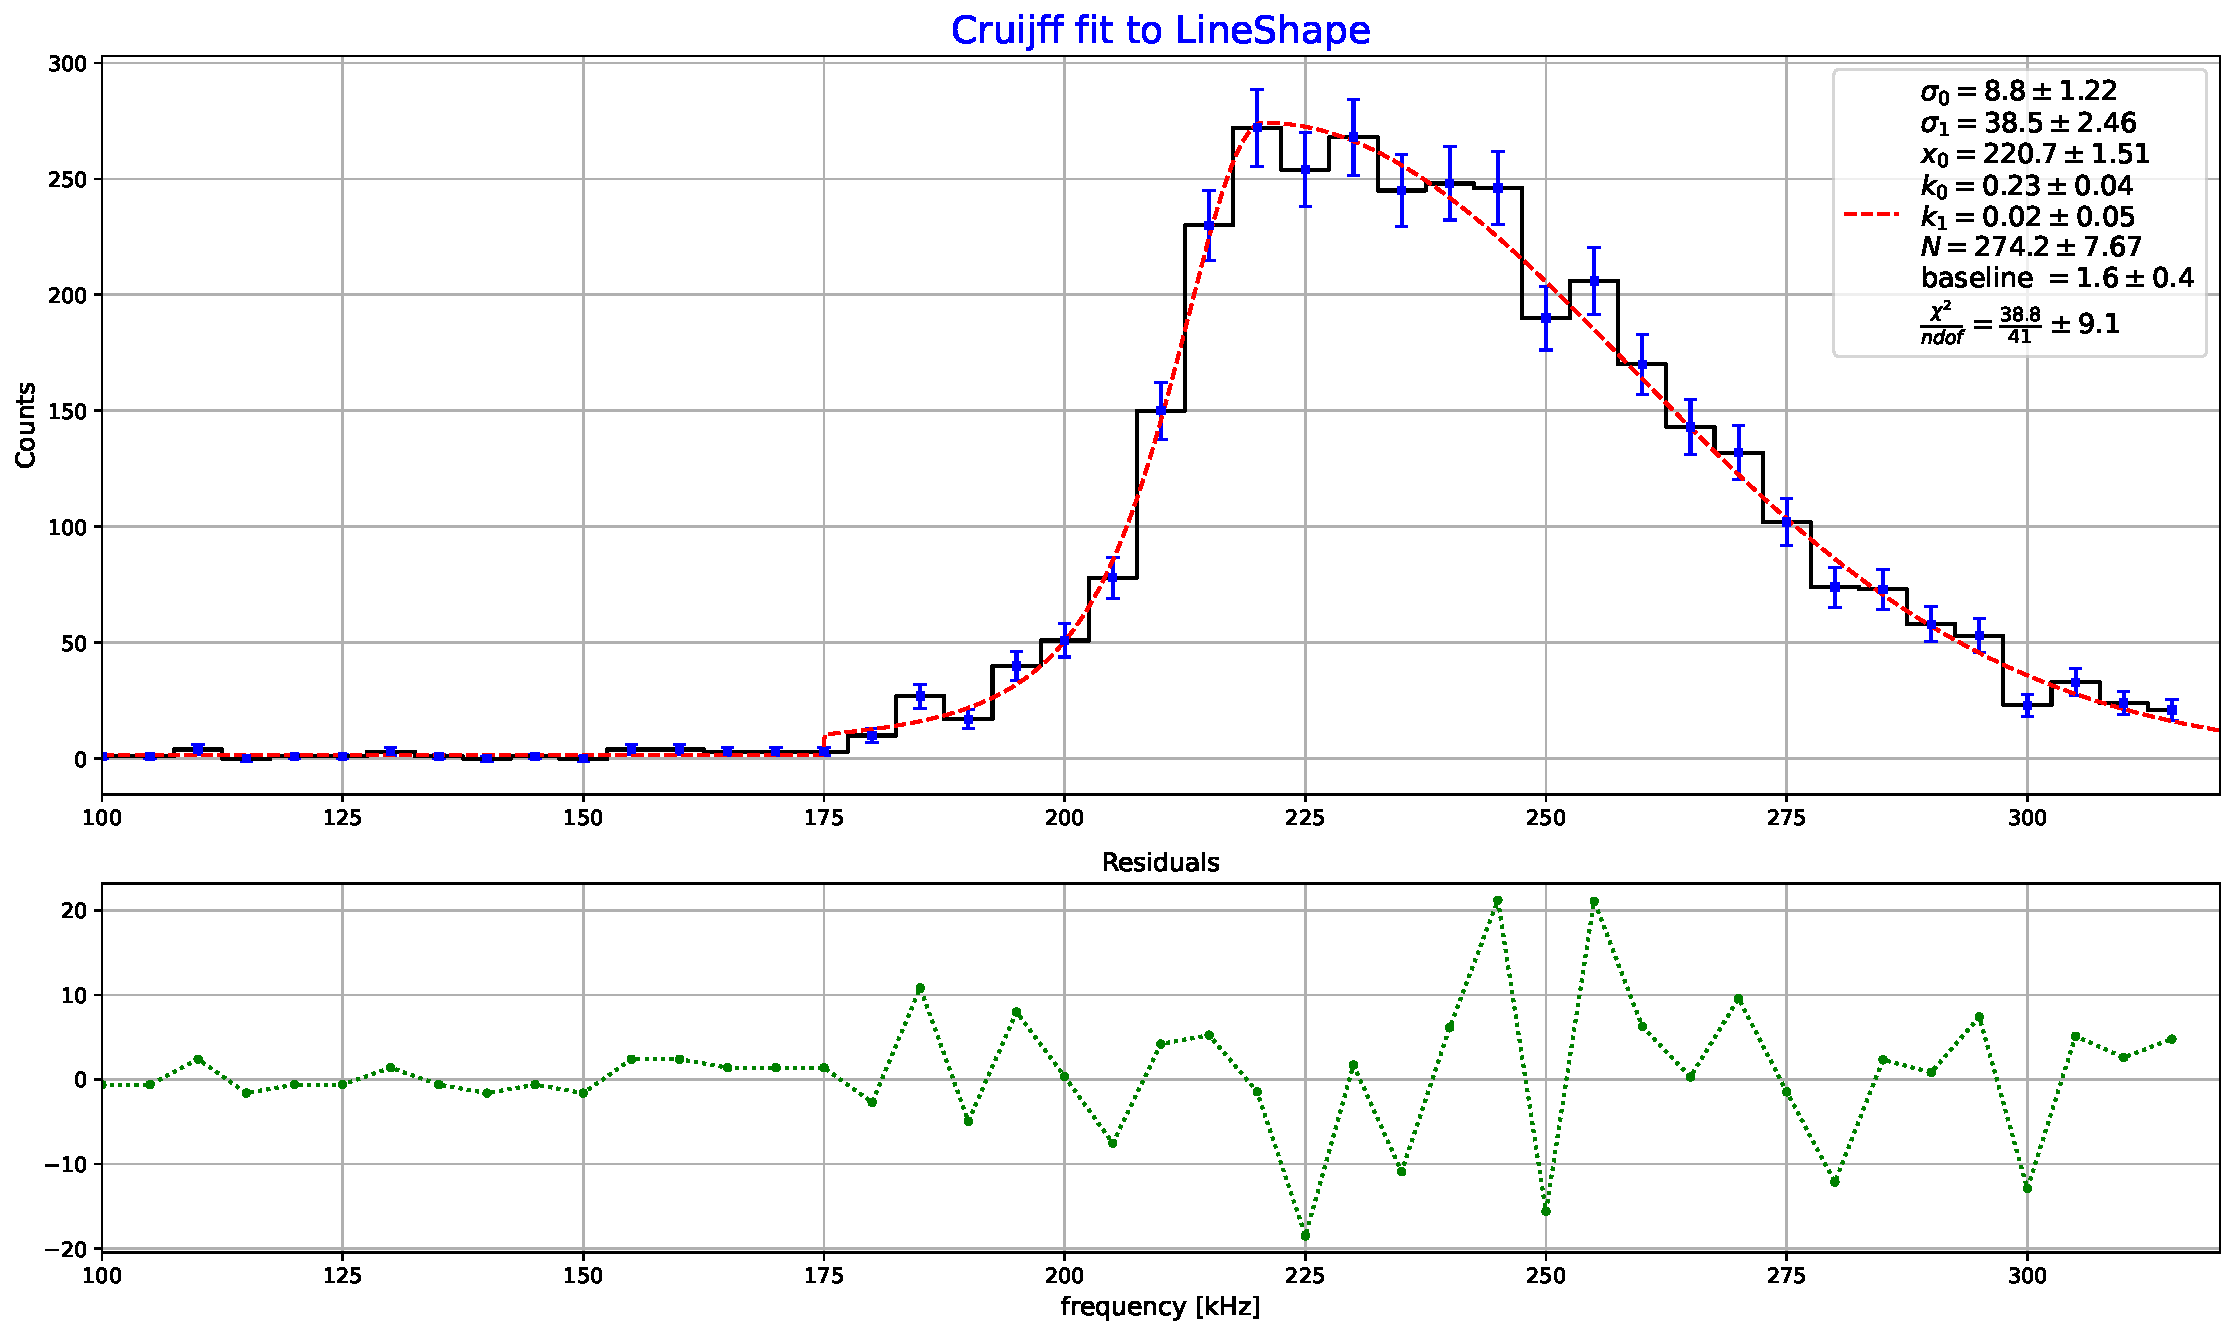
\includegraphics[width=0.8\textwidth]{TruncatedLineShape.pdf}
\end{figure}

\subsection{Discretization of the Line-Shape}

To generate the data, the baseline is removed from the model in equation \ref{eq:Cruiff}. The background events (which encompass both residual gas and cosmic events) and annihilation coming from the two transitions are generated separately and later combined together, to track the different type of annihilation. The procedure to generate the events from \ref{eq:Cruiff} needs an intermediate step, which we are referring to as \textit{discretization}. The model is discretized in a series of $50$ equally spaced points ( $y_{i}$), and then normalized so that: 

\begin{equation}
\sum_{i = 0}^{N = 50} y_{i} = 1
\end{equation}

In a real dataset, the length of the frequency sweep (aka, the number of frequencies measured) is less then the series of $50$ points used in the discretization. For the events belonging to frequencies that falls out of the sweep, they are assigned to the clearing sweep {\color{red}{(not done yet)}}.

\begin{figure}[hbtp]
\centering
\includegraphics[width=1\textwidth]{NormalizedLineshape.pdf}
\caption{Example of normalized Line-Shape, sampled with a frequency step of $\SI{5}{\kilo \hertz}$ with 50 frequency step. The red square dot represents the fraction corresponding to a sweep of $24$ steps. The values on the x axis are }
\end{figure}

Regarding the cosmic background, they are generated flat on each frequency {\color{red}{together with the background annihilations due to residual gas}}. 

\subsection{Radius Distributions}
 
 
\section{Variables of the }



\section{Onset Finding Algorithms: Definitions and Optimization}

\section{Magnetic field drift effects}

The magnetic field $\vec{B}$ in the anti-hydrogen trap can produce several effects that influence the hyperfine splitting measurement. For instance, magnetic field in-homogeneity could locally modify the frequency transition for a part of the trapped $\overline{H}$, broadening the spectroscopic line of the transition. Also
the variation of the magnetic field due to time influence both the onset frequency and shape of the \textit{cb} and \textit{da} transitions. The magnetic field drift $\vec{B}_{drift}$ (measured in $\SI{}{\kilo \hertz \second\tothe{-1}}$) is supposed to be constant over time, with magnitude of $ \simeq \SI{0.02}{\kilo \hertz \second\tothe{-1}}$ or equivalently $ \simeq \SI{70}{\kilo \hertz \hour\tothe{-1}}$.

The shape of the transition  is modified due to the fact that the experimental measurement at each frequency are made a different times. Denoting the transition as $\psi(t,f,\vec{B})$ where we have made the time, frequency and $\vec{B}$ dependence explicit, the measurement are at each frequency are given by:

\begin{eqnarray*}
f_{0}& : &\psi(f_{0},B(t))   \\
f_{1}& : &\psi(f_{1},B(t + \delta_{tstep})) = \psi(f_{0},B(t) - B_{drift} \cdot \delta t) \\
f_{2}& : &\psi(f_{2},B(t + 2\delta_{tstep})) = \psi(f_{0},B(t) - B_{drift} \cdot 2 \delta t)\\
... & ...
\end{eqnarray*}

In principle this effects could be simulated with a discretization of the line-shape which accounts for the explicit dependence over time. Despite this, for low magnitude of $B_{drift}$, the shift produced is of the order of $\SI{0.02}{\kilo \hertz \second \tothe{-1}} \cdot \delta t_{step} = \SI{0.16}{\kilo \hertz}$, having imposed $\delta t_{step} =\SI{8}{\second}$. The effect is relatively small compared to the frequency increment of $\SI{5}{\kilo \hertz}$ for each step. Despite this, since this effect accumulates over time, the biggest effect will occur for higher frequencies at the end of the sweep. For the very last been of the sweep, we expect to have $ \SI{0.16}{\kilo \hertz} \cdot 24  = \SI{3.84}{\kilo \hertz} $, where 24 is number of step in a single. In this case the result is comparable with the frequency sampling of 5 kHz, nevertheless this only modifies the shape of the right tail of the lineshape, with a negligible influence on the onset determination.

A more significant effects, which is considered in the simulation, is directly related to the change over time of the onsets frequencies. Since the onsets of the \textit{cb} and \textit{da} transition are measured at a different time, the hyperfine splitting of anti-hydrongen, measured as the difference between the two onsets, is directly influenced by the $B_{drift}$ effect. 

\begin{figure}[hbtp]
\centering
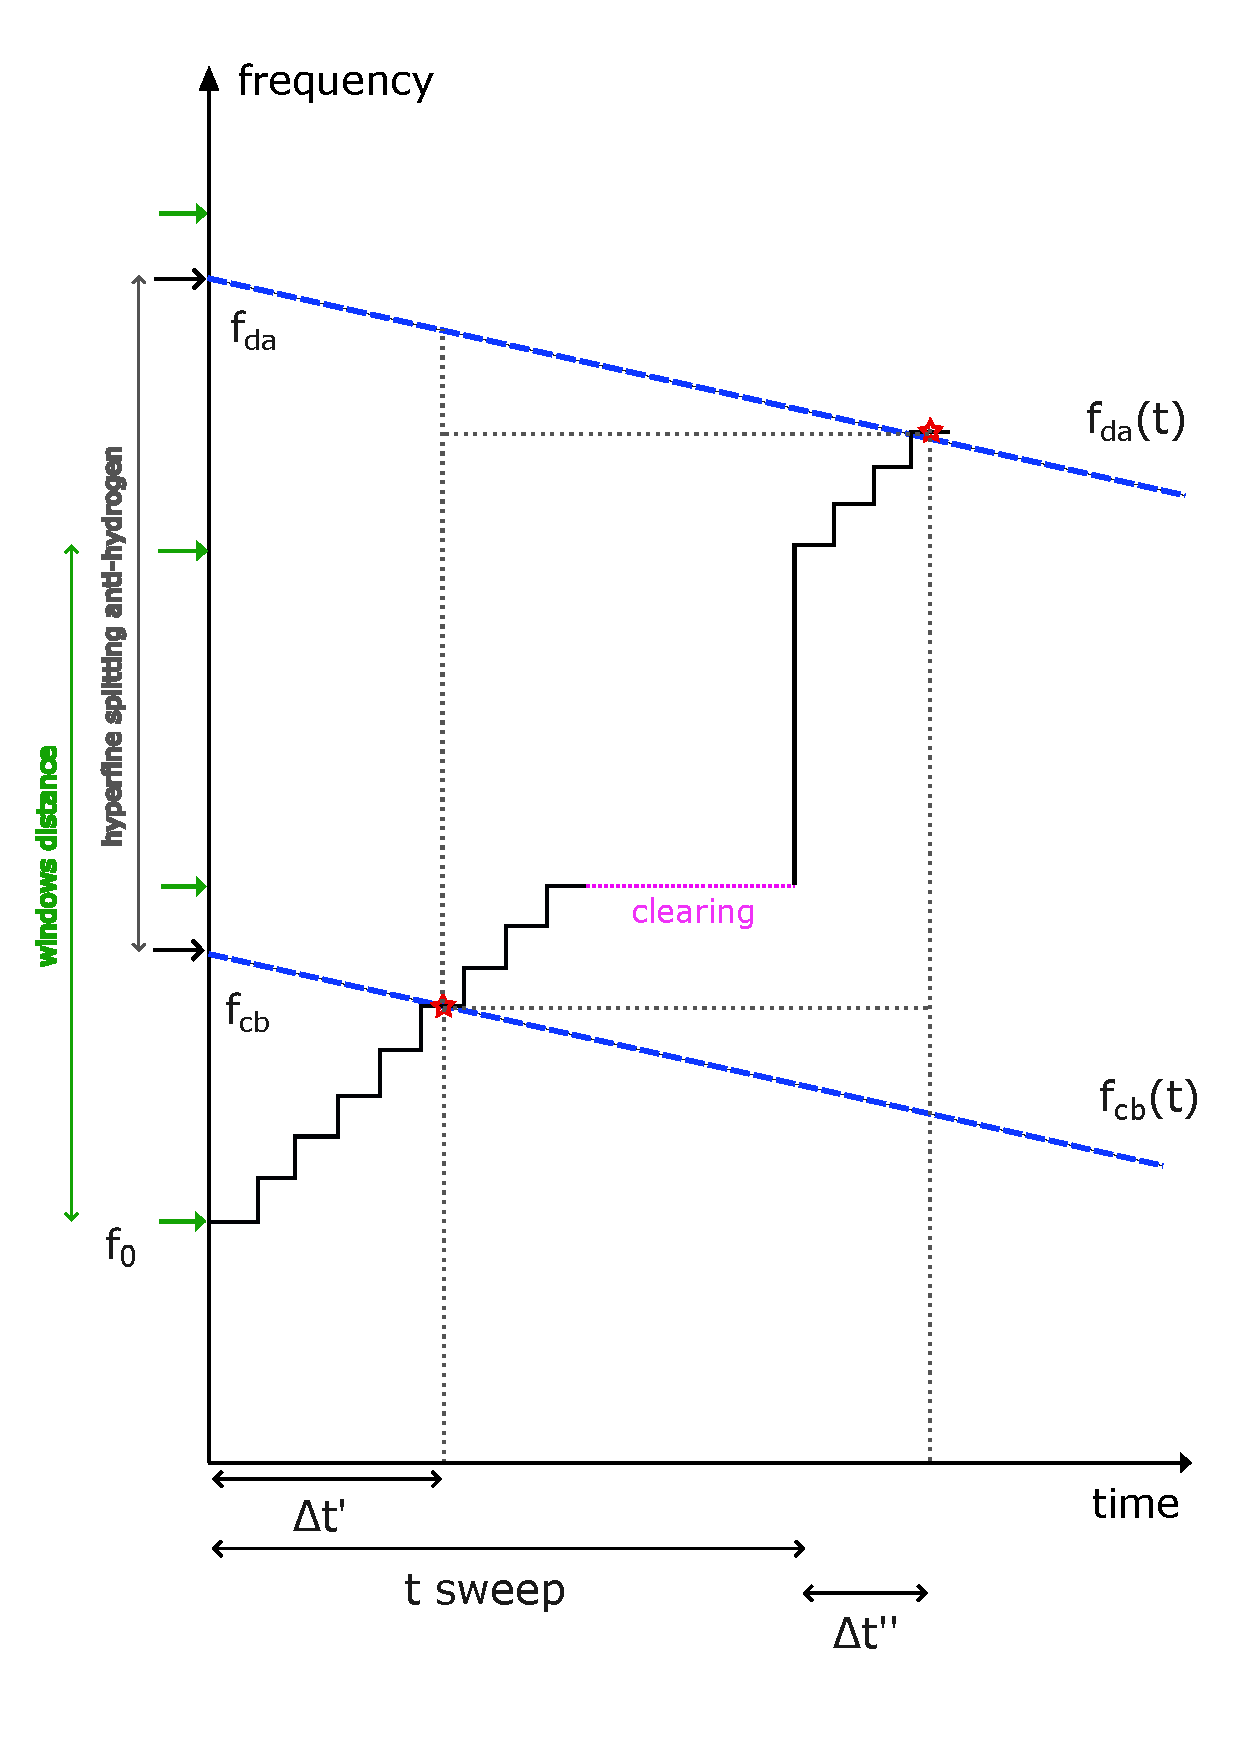
\includegraphics[scale= 0.60]{SchemeBdrift.pdf}
\caption{Scheme of Bdrift effects on onset determination}\label{fig:SchemeBdrift}
\end{figure}


A quantitative estimation of this effect is calculated from the scheme shown in figure \ref{fig:SchemeBdrift}. The onset \textit{cb} is found when the blue line (which represent the variation of the onset frequency given by the $B_{drift}$ effects) intersects the step by step rising frequency of the micro wave laser used to induce the transitions. Considering an ideal algorithm without uncertainty, this is equivalent to:

\begin{equation} \label{eq:cbOnset}
f_{0} + \dfrac{f_{step}}{t_{dwell}} \cdot \Delta t' = f_{cb}(t) = f_{cb} - B_{drift} \cdot \Delta t'
\end{equation}

Resolving this equation in the variable $\Delta t'$, the time at which the onset is found, gives:

\begin{equation}
\Delta t' = \dfrac{f_{cb} - f_{0}}{ \frac{f_{step}}{t_{dwell}} + B_{drift}}
\end{equation}

Substituting in $f_{cb}(t)$ gives the measured onset for the \textit{cb} transition:

\begin{equation}
f_{cb}(t = \Delta t') = f_{cb} - B_{drift} \dfrac{f_{cb} - f_{0}}{ \frac{f_{step}}{t_{dwell}} + B_{drift}}
\end{equation} 

The onset for \textit{da} transition can be found with the same method, although we have to consider an additional time interval made up by the last frequency steps of the \textit{cb} transition and the 16 clearing step. With this additional information we can derive the equivalent equation of the \ref{eq:cbOnset}

\begin{equation}
f_{0} + hfs +  \dfrac{f_{step}}{t_{dwell}} \cdot \Delta t'' = f_{da} -B_{drift} \cdot (t_{sweep} + \Delta t'') 
\end{equation}

where $hfs$ indicates the frequency distance between the two starting point of the sweep (equal to the hyperfine splitting of hydrogen). The time $\Delta t''$ is:

\begin{equation}
\Delta t'' = \dfrac{f_{da} - B_{drift} \cdot t_{sweep} - f_{0} - hfs}{ \frac{f_{step}}{t_{dwell}} + B_{drift}}
\end{equation} 

As before, substituting in $f_{da}$ gives the result:

\begin{equation}
f_{da} - B_{drift} t_{sweep} - B_{drift} \dfrac{( f_{da} - B_{drift} t_{sweep} - f_{0} - hfs)}{ \frac{f_{step}}{t_{dwell}} + B_{drift}}
\end{equation}

It is interesting now to study the difference between the two onset, which allows to identify quantitatively how much the $B_{drift}$ influence the measurement. 

\begin{equation} \label{eq:Systematiceffect}
\overline{hfs}_{measured} = \overline{hfs} - B_{drift} \cdot t_{sweep} - B_{drift}  \dfrac{(\overline{hfs} - hfs - B_{drift} \cdot t_{sweep})}{ \frac{f_{step}}{t_{dwell}} + B_{drift}}
\end{equation}

If the $B_{drift}$ are small compared to $\frac{f_{step}}{t_{dwell}}$, we can simplify the expression above, obtaining:

\begin{equation}
\overline{hfs}_{measured} = \overline{hfs} - B_{drift} \cdot \biggl(t_{sweep} + \frac{ \overline{hfs} - hfs}{\frac{f_{step}}{t_{dwell}}} \biggl) + \, B_{drift}^{2} \cdot \biggl( t_{sweep} \, \frac{t_{dwell}}{f_{step}} \biggl)
\end{equation}

two additional terms are present, one which is proportional to the magnetic field drift, and one proportional to the square.


\begin{figure}[hbtp]
\centering
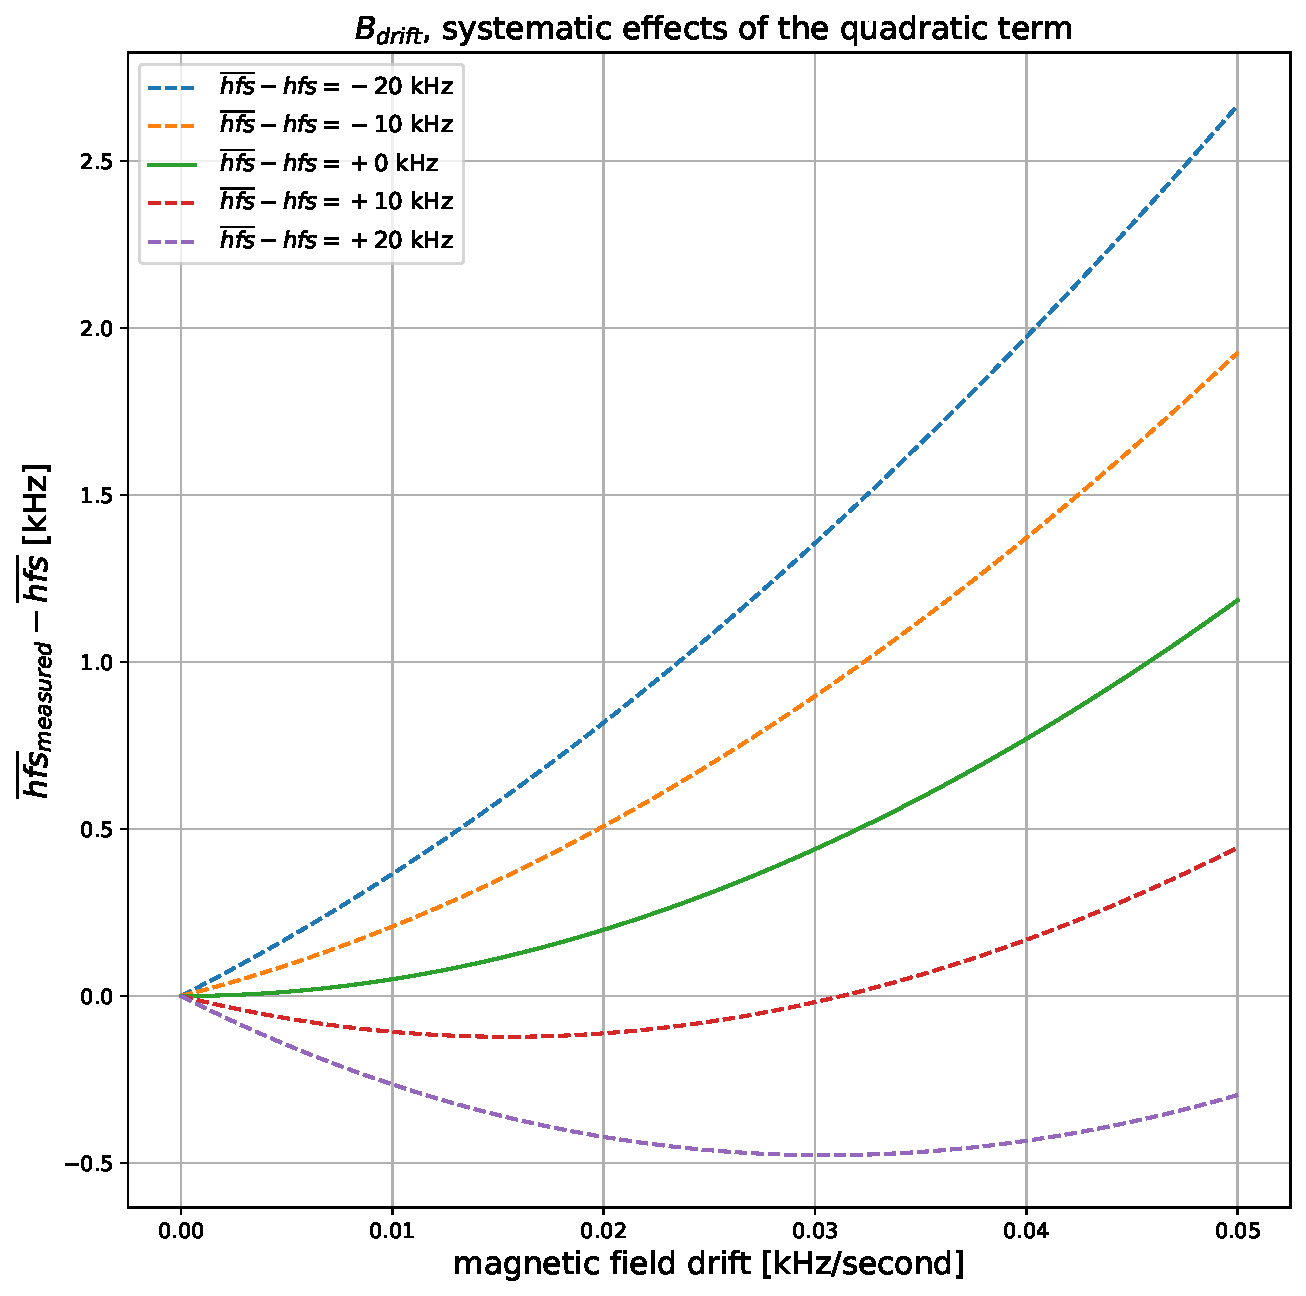
\includegraphics[width = 0.75\textwidth]{SecondOrderTerm.pdf}
\caption{Plot of the second order term of equation \ref{eq:Systematiceffect}. The $B_{drift}$ effects are computed for 5 different possible scenarios with a different hyperfine splitting of anti-hydrogen with respect to hydrogen ($\overline{hfs} - hfs$) }
\end{figure}


\section{Results}

\end{document}